%% ==============================
\chapter{\iflanguage{ngerman}{Derzeitiger Stand}{Current State}}
\label{sec:current_applications}
\subsection{Neurosurgery}
\label{sec:Neurosurgery}
The top layer of the brain, the cortex, is only 2-4mm thick and strongly folded, underneath of the cortex are thousands of nerve fibers. The surgeon has to be extremely careful to not damage any nerves due to false movement. \\
With the help of micro robotic systems the surgeon is able to operate much more accurate. He has also the possibility to manipulate tissue in narrow spaces which otherwise would be too risky to reach. This leads to the fact that micro robotic systems are widely adapted in the area of neurosurgery.\\
The tool tip is one of the most important part in micro surgery because it has the most contact to the tissue when moving to the desired position. It must not damage tissue. On the other side it also needs to be able to manipulate the tissue. One approach to handle this issue is tuning the stiffness of the tool. The tool doesn't consist of one stiff element (Fig: \ref{fig:stifftool}) but of multiple stiff elements connected by springs (Fig: \ref{fig:bendabletool}).
\begin{figure}[H]
    \centering
    \begin{subfigure}[b]{0.45\textwidth}
        
\includegraphics[width=\textwidth]{Figures/stiff_element.png}
        \caption{Stiff tool}
        \label{fig:stifftool}
    \end{subfigure}
    \qquad
    \begin{subfigure}[b]{0.45\textwidth}
        
\includegraphics[width=\textwidth]{Figures/spring_element.png}
        \caption{Semi flexible tool}
        \label{fig:bendabletool}
    \end{subfigure}
    \caption{Completely stiff and semi-flexible tools}\label{fig:logos}
\end{figure}
Another problem occurs when the tool shaft is not designed completely stiff. The control over the semi-flexible tool is harder as when using a completely stiff tool. This leads to issues when the tool head has to be moved in a small area. To counter this problem materials  which can be manipulated through heat, electricity or other influences are used for the springs. \\
This approach is described in a work of Yeongjin Kim et. al. \cite{StiffnessTuning}. They propose the use of a \grqq shape memory alloy (SMA) spring backbone that provides local stiffness control and a tendon routing configuration that enables independent segment locking \grqq \cite{StiffnessTuning}. The SMA is controlled by heat. When the alloy is heated up it is very stiff and if it is cooled down it is bendable. The team was able to control each segment independently, this allows more use cases. \\
The used springs are able to bend 45° which results in maximum angle between two elements of 90°. To ensure the SMA does not damage any tissue a flexible, smooth casing is used. The team around J. Desai used a second smother spring to cover the SMA (Fig. \ref{fig:springsbasedconstrucion}). Their backbone  consists completely of SMA. The stiff elements are disks and the bendable elements are springs between the disks (Fig. \ref{fig:springsbasedconstrucion}). Their prototype (Fig. \ref{fig:prototype}) is 65mm long and has an outer diameter of 12.6mm. This is relatively big for micro surgery but through the simple design it is easily possible to reduce the size of the tool. This tool was designed to remove brain tumors having a size of less than 40mm.
\begin{figure}[H]
    \centering
    \begin{subfigure}[b]{0.45\textwidth}
        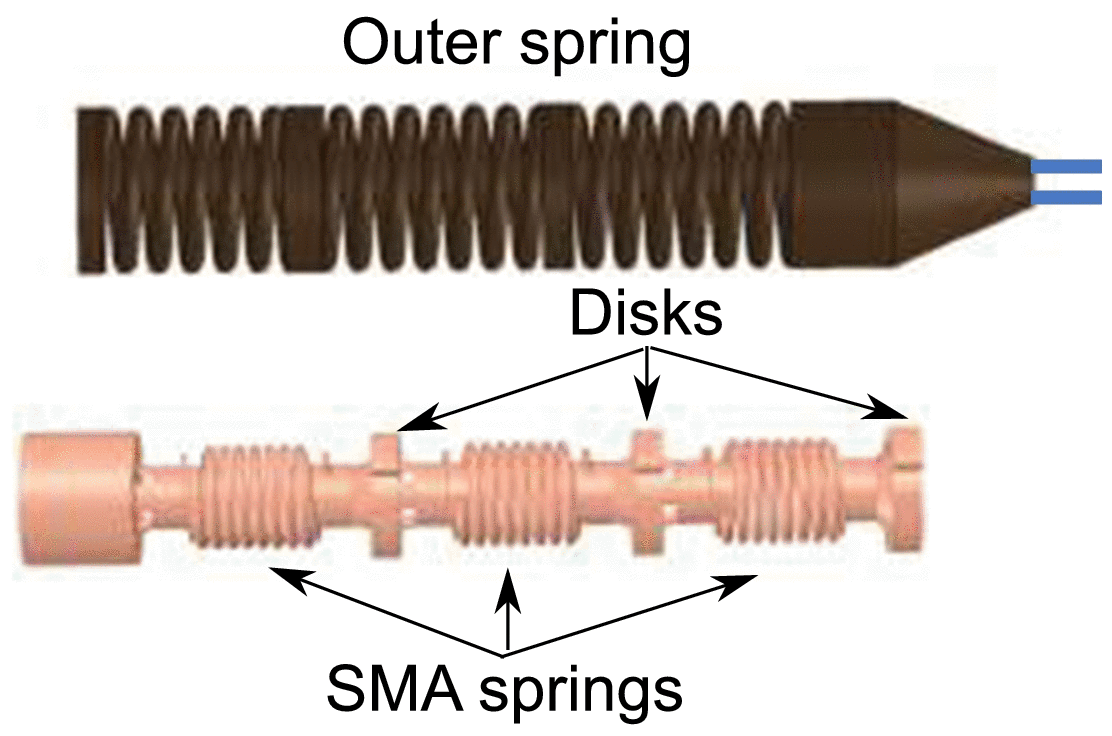
\includegraphics[width=\textwidth]{Figures/springbasedconstruction.png}
        \caption{Structure of the semi-flexible tool}
        \label{fig:springsbasedconstrucion}
    \end{subfigure}
    \qquad
    \begin{subfigure}[b]{0.45\textwidth}
        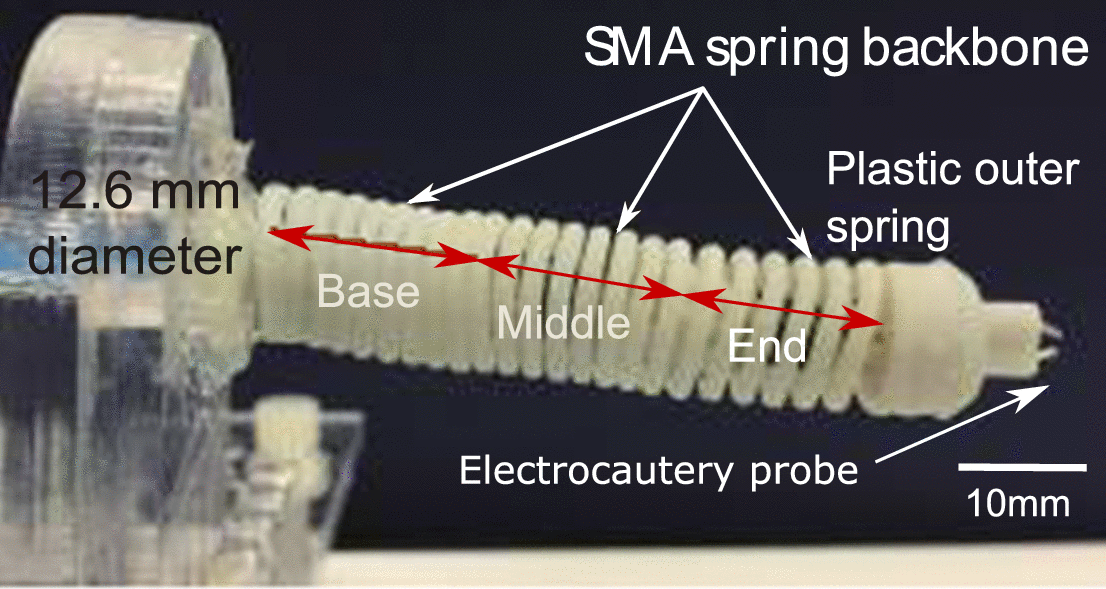
\includegraphics[width=\textwidth]{Figures/prototype.png}
        \caption{Prototype of a semi-flexible tool}
        \label{fig:prototype}
    \end{subfigure}
    \caption{Structure and prototype of the semi-flexible tool \cite{StiffnessTuning}}
    \label{fig:structure_prototype}
\end{figure}
With this tool the navigation to a tumor or other tissue to manipulate is possible. Now, there are some issues: first the creation of enough force in the small space to cut through the tissue, second the activation of the scissors.\\
The intuitive approach would be to use an electric cable inside the tool and to use electricity to close and open the scissors. This would need more space than wireless actuated and space is very valuable in a narrow space like the brain. That implicates the goal to  wireless activate the tool head. \\
It is necessary to cut through different kinds of tissue. For example to cut through rat liver 1.6N and 7.1N for sheep liver is needed, in contrast 2.5mN is needed for mouse brain \cite{ScissorActuation}. It is important to know that the required cutting force depends on the cutting speed and the cutting area. \\
O. Onaizah and E. Diller developed a working prototype (Fig. \ref{fig:scissor_prototype}) of a pair of scissors actuated by a magnetic field of 20mT \cite{ScissorActuation}. Therefore titanium is used for the blades and neodymium iron boron permanent magnets are clued onto the blades for closing the scissor. \\
An incremental part of the scissor is the joint of the two scissors, typical a pin joint is used. \grqq However, on the millimeter scale, this introduces a large amount of friction that tends to jam the actuation\grqq \cite{ScissorActuation}. So the team used a sandwich design (Fig. \ref{fig:scissor_design}) and used a spring of shape memory alloy to reopen the scissor. 
\begin{figure}[H]
    \centering
    \begin{subfigure}[b]{0.45\textwidth}
        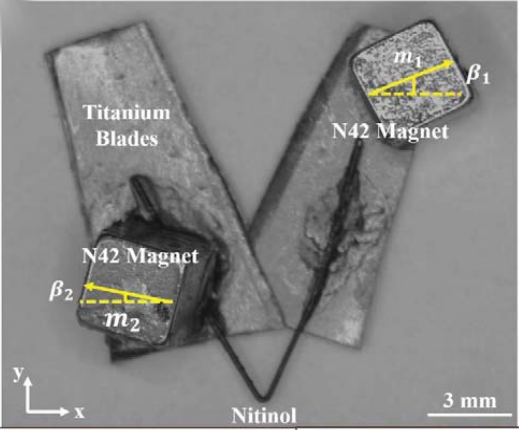
\includegraphics[width=\textwidth]{Figures/scissor_prototype.png}
        \caption{Prototype of wireless actuated scissors}
        \label{fig:scissor_prototype}
    \end{subfigure}
    \qquad 
    \begin{subfigure}[b]{0.45\textwidth}
        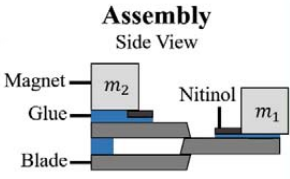
\includegraphics[width=\textwidth]{Figures/scissor_design.png}
        \caption{Design of the scissors}
        \label{fig:scissor_design}
    \end{subfigure}
    \caption{Prototype and design of wireless actuated scissors \cite{ScissorActuation}}
    \label{fig:scissors}
\end{figure}
\newpage
The prototype has a size of 15mm x 15mm when open and 15mm x 11mm when closed. They achieved a cutting force between 16 to 35mN with a magnetic field of 20mT. That would be enough for a rat brain but not nearly enough to manipulate liver tissue from a rat or sheep.\\
The torque of the scissors is calculated with: 
\begin{align*}
    \tau = m_{net} \times B = (m_1 * sin \beta_1 + m_2 * sin \beta_2) \times B \qquad \cite{ScissorActuation}
\end{align*}
$m$ is the magnetic torque of the magnets and $B$ is the applied magnetic flux density. \\
To increase the torque of the scissors a higher magnetic field to actuate the scissors or magnets with higher magnetic torque are required. Current studies have shown that it is possible to produce an external magnetic field with up to 400mT with a clinical sized coil system \cite{MagneticField}. That results in a torque of up to 1.5N. \\
Another issue is, the scissors are too big for micro surgery, this issue is already discussed from the team: \grqq The scissors can easily be scaled down \grqq \cite{ScissorActuation} due to the simplistic design of scissors. The down scaling of the scissors results in another problem. With reduced size also the magnetic torque of the permanent magnets would be reduced. A higher external magnetic field is required to achieve the same torque.

Another possibility to manipulate tissue is not to cut it but to tear it off. \\
A team from ETH Zurich proposed a prototype of such a milli gripper in their work (Fig. \ref{fig:gripper_prototype}) \cite{MilliGripper}. Their approach was to use a simple design made of the gripper, a coil and a neodymium magnet (Fig. \ref{fig:gripper_design}). If a magnetic field is applied to the gripper, current is inducted into the coil. The magnetic interaction between the coil and the permanent magnet forces the gripper jaws to close or open, depending on the direction of the external magnetic field. They also used the permanent magnet to navigate the gripper. The prototype is designed to fit in a capsule with inner diameter of 8mm. The team tested the prototype with a porcine liver. They were able to remove parts of the liver. Their design has no sharp edges and corners, so it is less probable to injure tissue in contrast to the wireless actuated scissors which having sharp edges.
\begin{figure}[H]
    \centering
    \begin{subfigure}[b]{0.45\textwidth}
        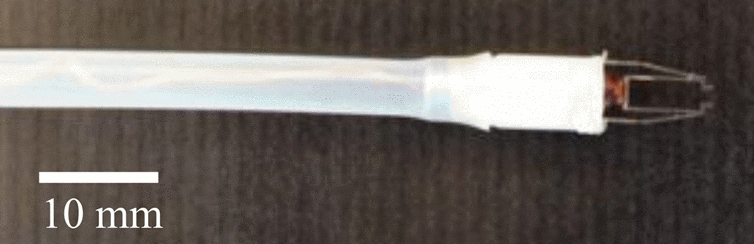
\includegraphics[width=\textwidth]{Figures/prototype_gripper.png}
        \caption{Prototype of the milli gripper}
        \label{fig:gripper_prototype}
    \end{subfigure}
    \qquad
    \begin{subfigure}[b]{0.45\textwidth}
        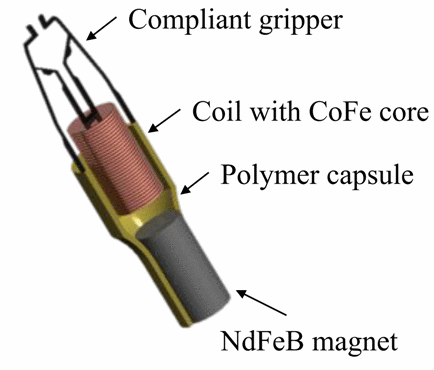
\includegraphics[width=\textwidth]{Figures/structure_gripper.png}
        \caption{Design of the milli gripper}
        \label{fig:gripper_design}
    \end{subfigure}
    \caption{Prototype and design of the milli gripper \cite{MilliGripper}}
    \label{fig:gripper}
\end{figure}
These different prototypes can be combined to create a tool to remove a brain tumor. One tool used in micro surgery is the CorPath GRX (Fig. \ref{fig:corindusCorPath}).  A study, conducted by a team from the Department of Neurological Surgery and Neurological Institute in Houston, evaluated the feasibility of a minimal invasive robotic system to heal neurovascular disorder \cite{Neurovascular}. They tested the robotic system in a flow and a porcine model. No technical complications occurred and the deployment of the platform was successful.  
\begin{figure}[H]
    \centering
    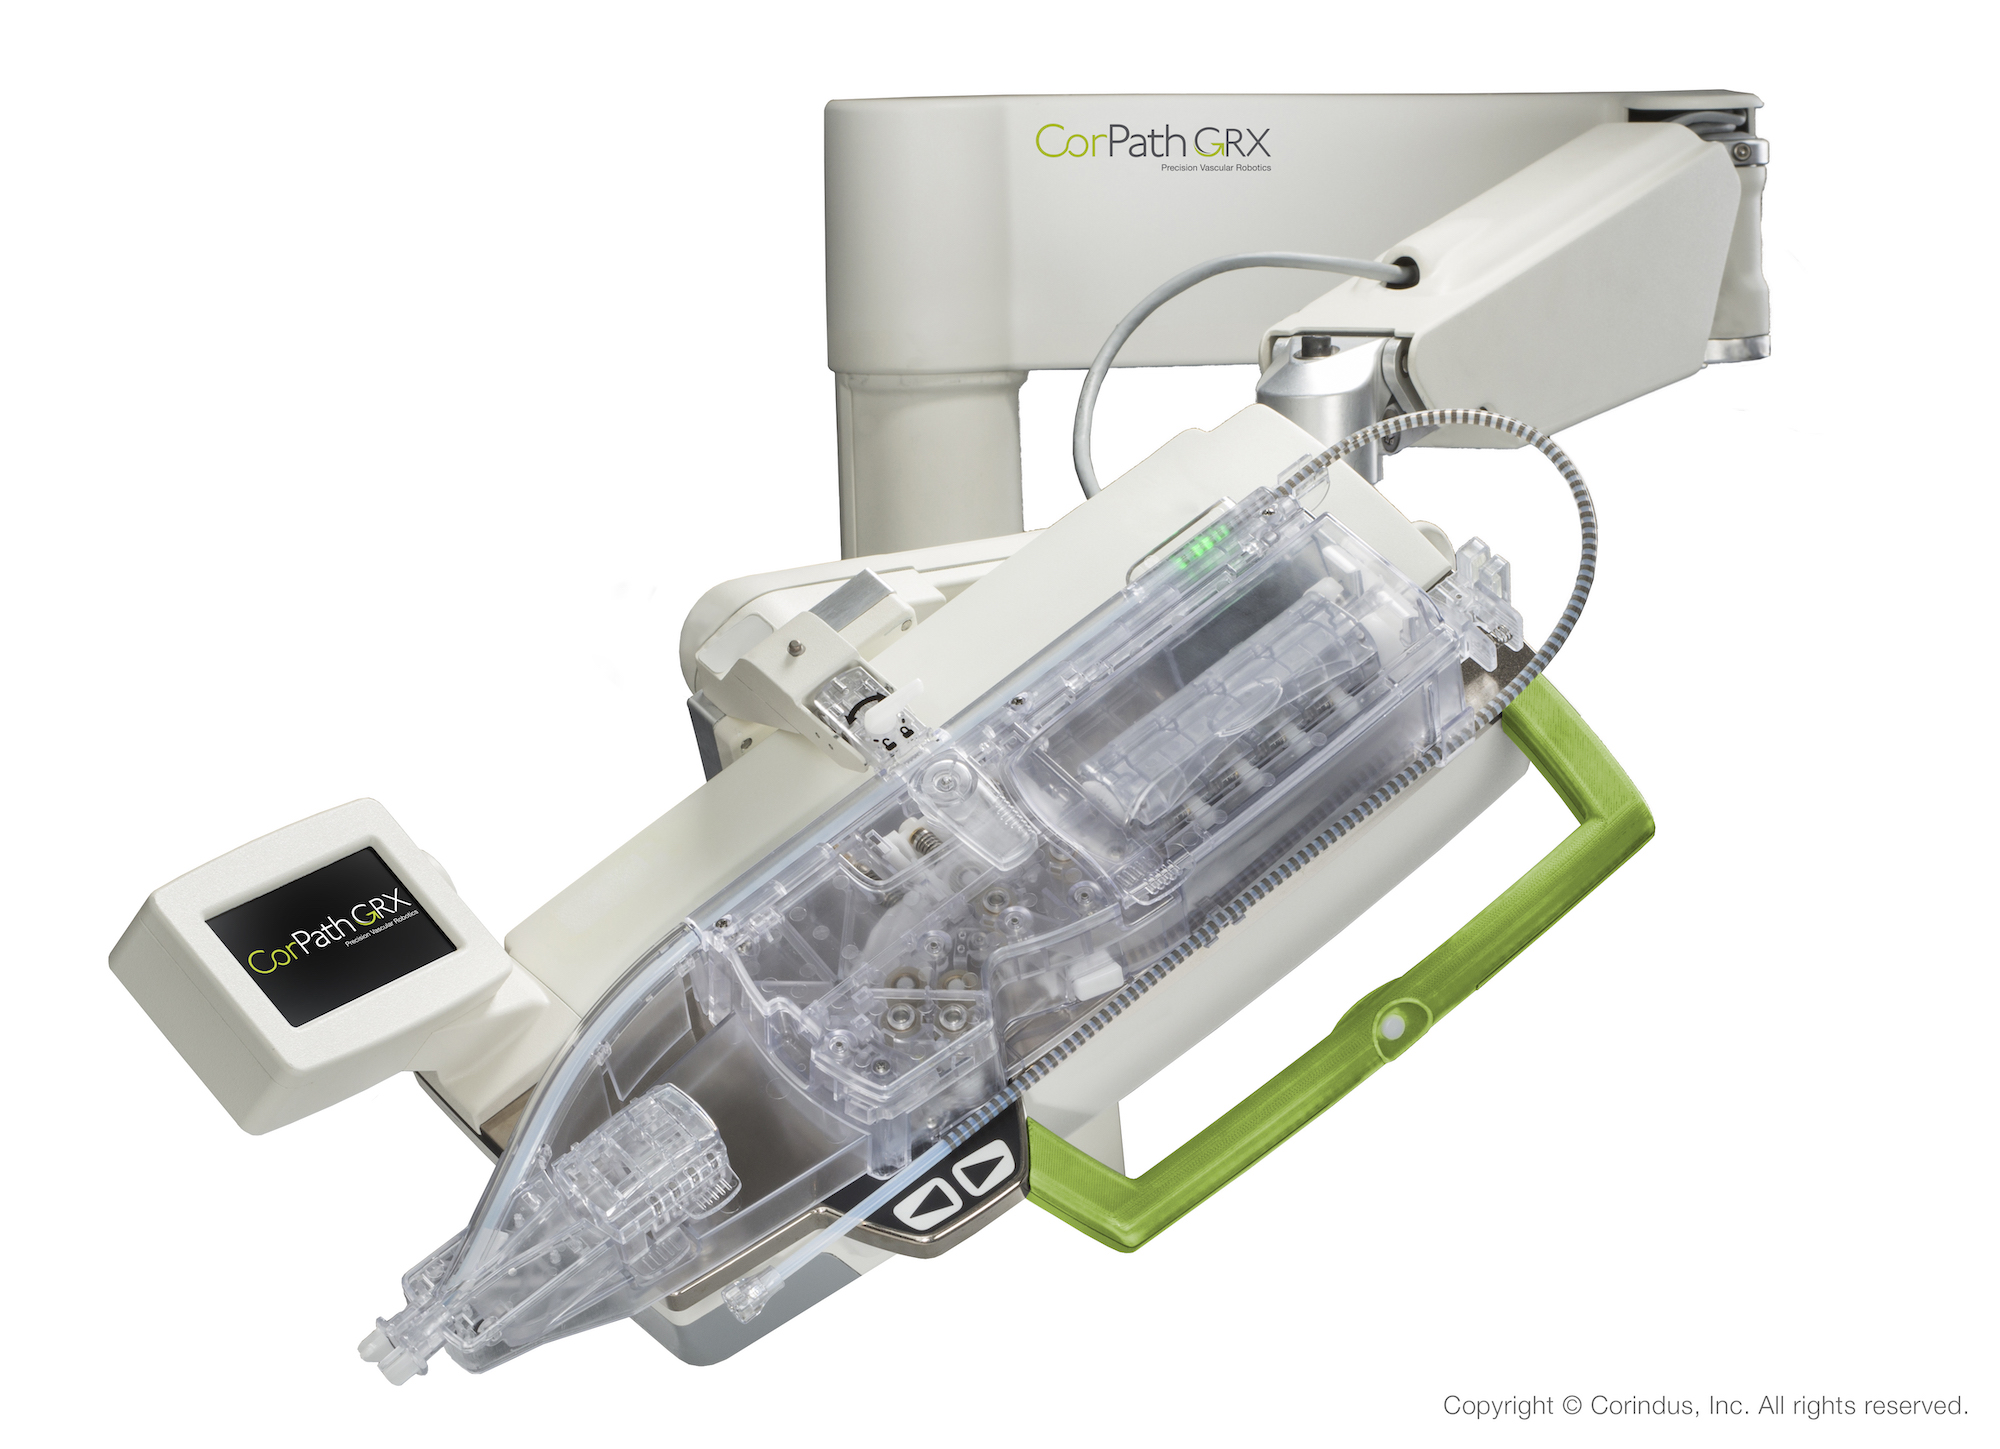
\includegraphics[width=0.5\textwidth]{Figures/CorindusCorPathGRX_1.jpg}
    \caption{Corindus CorPath GRX}
    \label{fig:corindusCorPath}
\end{figure}
Originally CorPath GRX was developed for peripheral vascular intervention. It was shown such a robotic system is not only suitable for one area of surgery but for many others too like in this case neurovascular disorder. Also the combination of the different prototypes can not only be used for removing brain tumors. It could also be used for surgeries in the stomach area or for heart surgeries.

\subsection{Ophthalmic}
\label{sec:eyesurgery}
Another field where miniature robot systems and micro surgery is very useful is the the area of Ophtalmic. The tool proposed in \ref{sec:Neurosurgery} is a semi flexible tool. But the goal for eye surgery is to reduce the force applied on the retina as much as possible because the risk of retinal tears are reduced with less applied force. A study has shown that the use of a complete flexible tool reduces the applied force by up to 37\% \cite{flexibleRetina}. They compared straight instruments to flexible ones. Therefore they used tools with a diameter of 0.8mm and measured the displacement of the fiber network in the eye when manipulating the retina. The maximum displacement of the mesh was reduced by up to 50 \%, less if more force on the tool is applied. The differences are shown in figure \ref{fig:displacement}. The manual control of an complete flexible and very thin tool is hard for the surgeon. But it can be used by a robotic system which is able to move the tool more accurate and steady. A flexible tool is the perfect addition to the toolbox of a miniature robotic system.
\begin{figure}[H]
    \centering
    \begin{subfigure}[b]{0.3\textwidth}
        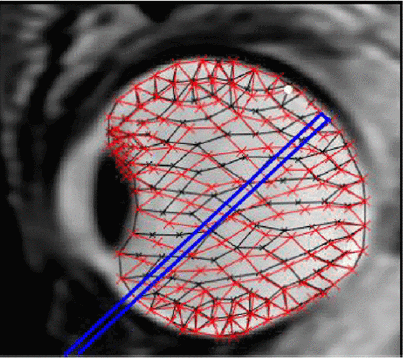
\includegraphics[width=\textwidth]{Figures/displacement_stiff.png}
        \caption{Displacement of the fiber network for a straight tool}
        \label{fig:displacement_stiff}
    \end{subfigure}
    \qquad \qquad
    \begin{subfigure}[b]{0.3\textwidth}
        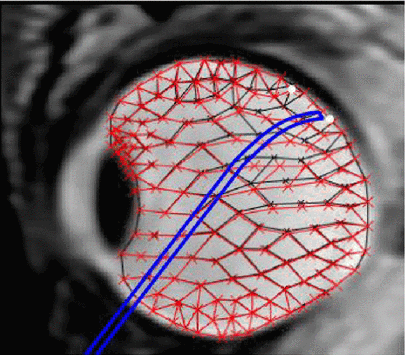
\includegraphics[width=\textwidth]{Figures/displacement_flex.png}
        \caption{Displacement of the fiber network for a flexible tool}
        \label{fig:dispalcement_flex}
    \end{subfigure}
    \caption{Displacement of the fiber network in the eye when manipulating the retina with different tools. The initial mesh is shown in black and the displacement is shown in red. An exerted force of 10Nm is assumed \cite{flexibleRetina}}
    \label{fig:displacement}
\end{figure}
\newpage
An often used tool in robotic surgery is the Da Vinci Surgical System and it has many use cases \cite{davinci}. For example it can be used for ocular micro surgeries \cite{davinciOcularSurgery}. The Da Vinci System can be equipped with the Hexapod Surgical System (HSS) to overcome limitations like a limited motion area \cite{davinciWithHSS}. This upgrade enables the robotic platform to perform micro surgeries. 
The retinal vein occlusion (RVO) is a blinding disease for which a manual surgery is considered too risky because it is necessary to dissolve the occlusion by injecting anticoagulant directly into the blocked vein. This procedure is nearly impossible to perform manually, because the vein is 100\textmu m thick \cite{veincannulation}. The team from the university hospitals Leuven has shown that it is technically \grqq  feasible to safely inject an anticoagulant into a 100 \textmu m-thick retinal vein of an RVO patient for a period of 10 min with the aid of the presented robotic technology and instrumentation\grqq \cite{veincannulation} and therefore to heal an RVO patient with a miniature medical robotic system.

\subsection{Pregnancy help}
\label{sec:birthhelp}
Miniature robotic systems cannot only be applied in the area of surgeries but also for directed movement in the human body. For example robotic systems can be used for colonoscopy \cite{colonoscopy} or the transfer of an embryo into an suitable area of implantation \cite{embryoTransfer}. \\
If expecting parents decided to use assisted reproductive technology, the reasons for failure of pregnancy would be low uterine receptivity or an ineffective embryo transfer. A team from Japan tried to minimize the failure rate through an ineffective embryo transfer. They used a robotic system to deliver the embryo into a suitable area and to control the position of the embryo during implantation to counter the problem of the embryo floated out. The embryo is inserted into the micro robot (diameter: 2mm) which is attached to a catheter (Fig. \ref{fig:et_robot_design}). The catheter is inserted into the uterus where the micro robot is detached from the catheter and then magnetically guided to the a suitable area of implantation. Arrived in the desired location, the micro robot mechanically keeps the embryo in the suitable area (Fig. \ref{fig:et_action}). When the embryo is implanted the guiding magnet is removed and the micro robot is caught with the catheter and removed from the uterus. 
\begin{figure}[H]
    \centering
    \begin{subfigure}[b]{0.45\textwidth}
        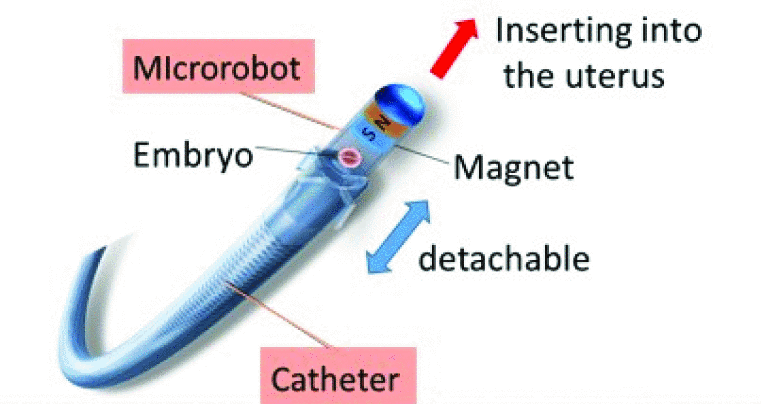
\includegraphics[width=\textwidth]{Figures/embryotransfer_robot.png}
        \caption{Design of the robotic system for embryo transfer}
        \label{fig:et_robot_design}
    \end{subfigure}
    \qquad
    \begin{subfigure}[b]{0.45\textwidth}
        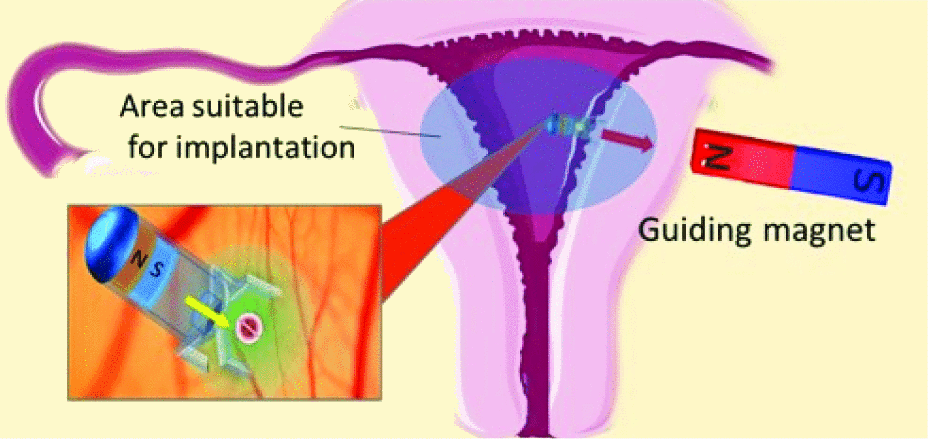
\includegraphics[width=\textwidth]{Figures/embryotransfer_action.png}
        \caption{Embryo transferring micro robot in action}
        \label{fig:et_action}
    \end{subfigure}
    \caption{Embryo transfer with micro robot \cite{embryoTransfer}}
    \label{fig:et}
\end{figure}
The embryo transfer method was tested with a female reproductive organ model. The tests confirmed the validity of the proposed miniature robotic system but further tests are pending. \cite{embryoTransfer}
